%%%%%%%%%%
% CH5 %
%%%%%%%%%%

\chapter{Les défauts cristallins}
\section{Introduction}
	Le cristal parfait constitue l'état idéal d'un matériau cristallin (énergie interne minimale). Cependa,t dans les cristaux réelles, il y a des imperfections et défauts qui font qu'ils ne sont jamais idéaux. A chaque défaut correspond un excès d'énergie libre par rapport à l'état d'énergie libre minimum. L'ensemble des défauts constitue la \textbf{microstructure}. Certaines propriétés des matériaux sont déterminées par cette microstructure. On distingue trois type de défauts : Les défauts ponctuels (dimension 0), linéaires (dimension 1) et bidimensionnels (dimension 2). 
	
\section{Les défauts ponctuels}
	\begin{wrapfigure}[3]{r}{5cm}
	\vspace{-5mm}
	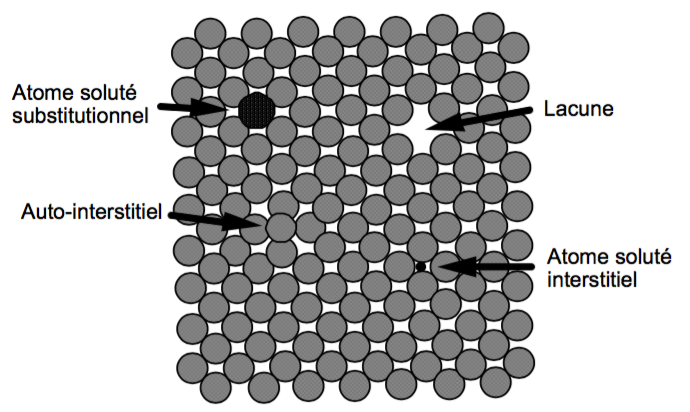
\includegraphics[scale=0.4]{ch5/1}
	\end{wrapfigure}
	Voici la liste des défauts qu'on rencontre dans les cristaux monoatomiques :
	\begin{enumerate}
		\item Les lacunes : absence d'atome sur un site du cristal
		\item Les auto-interstitiels : atome dans une position qui n'est pas un site du cristal
		\item Les interstitiels : atome étranger dans un site qui n'appartient pas au cristal
		\item Les substitutionnels : atome étranger qui remplace un atome du réseau hôte 
	\end{enumerate}
	Dans les cristaux multiatomiques comme les cristaux ioniques, les défauts ponctuels sont plus complexes (on doit maintenir la neutralité électrique). Le déplacement des ions entraîne la formation de paires de défauts voisins : 
	\begin{enumerate}
		\item Paires de \textbf{Schottky} : deux lacunes de nature différente
		\item Paires de \textbf{Frenkel} : une lacune et l'interstitiel correspondant
\end{enumerate}	 
Nous n'approfondissons pas plus. 

	\subsubsection{Les lacunes et les auto-interstitiels}
			Intéressons-nous à la variation de densité avec la température. En première approximation, une lacune augmente l'enthalpie du cristal d'une valeur correspondant au nombre de liaisons devenues insatisfaites. Soit $\Delta H_1$ l'enthalpie de formation d'une lacune et $\Delta S_1$ l'augmentation d'entropie due à la présence de lacune. On a alors la relation 
			\begin{equation}
				\Delta G_1 = \Delta H_1 - T\Delta S_1
			\end{equation}
			Si $N_t$ est le nombre de sites du cristal et $N_1$ le nombre de lacunes, la concentration en lacunes vaut $C_1 = \frac{N_1}{N_t}$ et s'exprime comme
			\begin{equation}
				C_1 = \exp \left( -\frac{\Delta G_1}{k_B T} \right) = \exp \left( \frac{\Delta S_1}{k_B} \right)\exp \left( -\frac{\Delta H_1}{k_B T} \right)
			\end{equation}
			La relation montre qu'il y a toujours une certaine concentration de lacunes qui augmente avec la température. Pour illustrer, dans une maille CFC l'énergie de formation vaut $1\, eV$. On calcule alors que la concentration à $300\, K$ vaut environ $10^{-22}$ alors qu'à $1300\, K$ elle passe à $10^{-5}$, c'est impressionnant ! En pratique, la présence de lacune permet aux atomes voisins de sauter et d'ainsi déplacer la lacune sur le réseau. C'est comme ça qu'est gouverné la mobilité des atomes dans le réseau. \\
			Le principe est le même pour les auto-inerstitiels sauf que leur enthalpie de formation est 4 fois plus grande (dans une CFC) que celle des lacunes, menant à une concentration négligeable à toute température. Le changement de concentration avec la température est permis par l'émission de lacunes par des \textbf{sources} ou leur absorption par des \textbf{puits}. 
			
	\subsection{Les sites interstitiels dans les structures cubiques}
		\begin{wrapfigure}[6]{l}{7cm}
	\vspace{-5mm}
	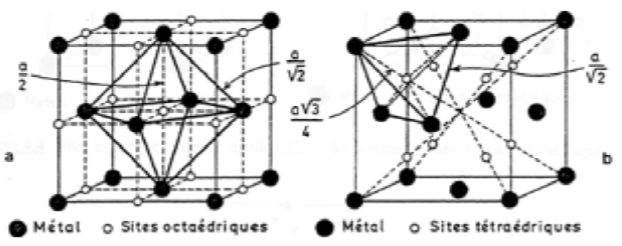
\includegraphics[scale=0.6]{ch5/2}
	\end{wrapfigure}
	On se rappelle du chapitre sur les structures CFC, CC et HC, qui sont celles de la plupart des métaux purs. Elles sont formés par l'empilement de sphères dures en contact les unes avec les autres. Comment les atomes de petite taille tape l'incruste ? On représente les CFC et CC comme un cube avec un atome à chaque sommet + un atome au milieu de chaque face pour le CFC et un atome au centre du cube pour le CC. \\
	Notons $R_A$ le rayon des sphères dures et étudions la forme géométrique représenté ci-contre (CFC). On trouve pour le \textbf{CFC} deux types de sites : 
	\begin{enumerate}
		\item des sites \textbf{octaédriques}, délimités par 6 atomes occupant les sommets d'un octaèdre
		\item des sites \textbf{tétraédriques}, définis par 4 atomes au sommet d'un tétraèdre
	\end{enumerate}
	Les deux types de polyèdres sont réguliers. Les sites octaédriques occupent le centre du cube et les milieux des arrêtes. Il y a un total de 4 sites octaédriques par maille (1 au centre + 12/4 aux arrêtes). Le rayon $R_0$ laissé à l'atome étranger vaut $0.414\, R_A$. Il y a 8 sites tétraédriques par maille (un huitième du cube = site). Le rayon libre dans ce cas est de $R_T = 0.225\, R_A$. On voit donc que l'octaédrique laisse un plus grand espace aux étrangers. \\
	\begin{wrapfigure}[6]{r}{7cm}
	\vspace{-10mm}
	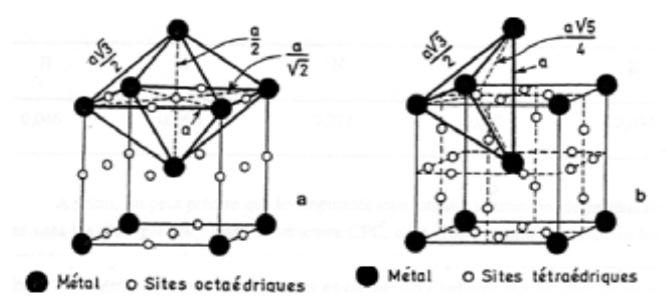
\includegraphics[scale=0.6]{ch5/3}
	\end{wrapfigure}
	Dans le cas de la structure \textbf{CC}, les polyèdres ne sont PLUS réguliers. Les sites octaédriques occupent les centres des faces, ainsi que le milieu des arrêtes. La distance du centre aux quatre coins du carré est plus grande que la distance entre les sommets de la pyramide. On a ainsi un rayon disponible de seulement $0.155\, R_A$ entre les sommets de la pyramide alors que dans la direction des 4 cotés du triangle on est à $0.633\, R_A$. Les sites tétraédriques se trouvent sur les faces du cube à mi-distance entre deux sites octaédriques. Il n'est pas régulier mais on peut y inscrire une sphère de rayon $0.211\, R_A$.
	
	\subsubsection{Solubilité}
		Pour qu'un atome étranger ne déforme pas le réseau, il faut que son rayon soit inférieur à $R_0$ ou $R_T$. Les seuls atomes de tailles suffisamment petites capable d'entrer en solution d'insertion sont $H,N,O,C$ et $B$. En fait, seul l'hydrogène est assez petit, les autres provoquent une distorsion du réseau. Les impuretés se placeront dans les interstices les plus grands. Dans la maille CFC sela correspond aux sites octaédriques alors que dans la CC c'est plus complexe dû à l'asymétrie des sites. Cependant, on observe qu'ils se placent préférentiellement dans les octaédrique, sûrement dû au seul contact avec deux atomes (distances entre 4 côtés du carré grands) alors que le tétraédrique en induit 4. \\
	On peut prévoir que la solubilité sera d'autant plus grande que la distorsion du cristal est faible. En effet, l'énergie de distorsion est une contribution positive à l'enthalpie libre du cristal. Si cette énergie devient trop grande, les nouvelles impuretés auront tendance à former un solide distinct de l'original. On en conclu que la solubilité des interstitiels est plus grande dans une CFC que dans une CC, alors que le volume totale des interstices est plus grand dans le CC mais leur nombre plus grand fait qu'ils sont plus petit. \\
		
		\begin{wrapfigure}[9]{r}{7cm}
	\vspace{-10mm}
	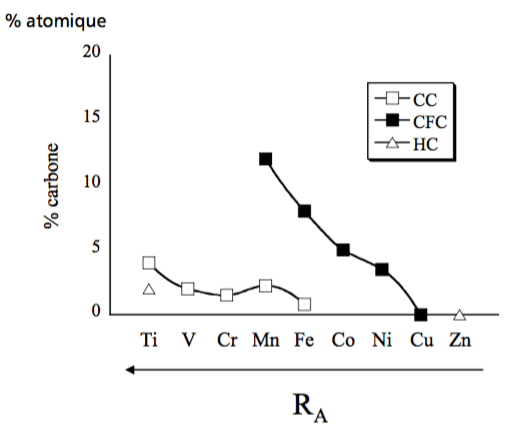
\includegraphics[scale=0.6]{ch5/4}
	\end{wrapfigure}
		Le cas du fer est particulièrement intéressant car il présente une structure CFC (austénite) à haute température et une structure CC (ferrite) à basse température. Les aciers sont issus de la combinaison de fer et de carbone (max 2\% en poids). La solubilité du carbone dans la structure CFC sera plus grande que dans la structure CC. Lors du réchauffement, tout le carbone présent dans les aciers peut entrer facilement en solution avec l'austénite. Mais lors du refroidissement, le carbone sera en excès, donnant lieu à un précipité cristallin différent qui est dans les cas les plus simple un carbure de fer $Fe_3C$ (cémentite). Ces précipités affectent les propriétés mécaniques de l'acier et leur taille et forme dépendent sensiblement des conditions de refroidissement de l'acier. \\
		Dernièrement, il n'y a pas que le rayon atomique qui compte. En effet, une affinité chimique élevé entre l'élément interstitiel et l'élément métallique favorise la précipitation de composés distincts, limitant ainsi la teneur de l'élément en solution solide. C'est ainsi qu'on ne retrouve pratiquement pas d'$O_2$ dans le fer en raison de l'oxydation, alors que le rayon est inférieur à celui du carbone. 

\section{Les défauts linéaires : les dislocations}
	\subsection{Le concept de dislocation}
	Ce sont, pour l'essentiel, les propriétés des dislocations qui gouvernent les phénomènes de déformation plastique des matériaux cristallins. La dislocation apparaît dans un matériau lorsqu'une partie du matériau se déplace par rapport à l'autre par \textbf{glissement} le long d'un plan cristallin. Elle désigne le défaut linéaire à la frontière entre les deux parties. 
	
	\newpage
	\subsubsection{Dislocation coin}
	\begin{wrapfigure}[12]{l}{4cm}
	\vspace{-5mm}
	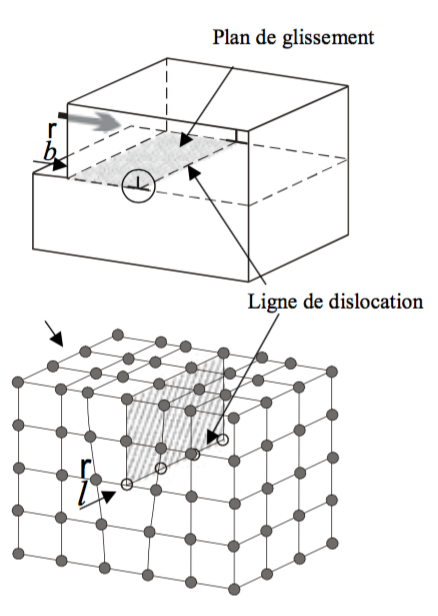
\includegraphics[scale=0.5]{ch5/5}
	\end{wrapfigure}
	Une partie du cristal est supposé s'être déplacé par rapport à l'autre sur une \textit{distance égale à la distance séparant deux noeuds équivalents du réseau}. Le glissement se fait suivant une direction parallèle à une direction du réseau, le long d'un plan particulier. Le \textbf{vecteur de Burger} $b$ représente cette direction. Aucun défaut n'est crée le long du plan de glissement. Cependant, une ligne de défaut se crée à la frontière entre la partie du plan qui se déplace et l'autre. On l'appelle \textbf{dislocation coin}. Le défaut peut être représenté comme étant situé àau voisinage de l'arête d'un demi-plan supplémentaire inséré entre deux plans du réseau. La partie la plus déformée sera alors appelé \textbf{coeur de la dislocation}. L'orientation de la ligne de dislocation peut être décrite par un vecteur unitaire $l$. Dans le cas d'une dislocation coin, $l$ et $b$ sont perpendiculaires. 
	\subsubsection{Dislocation vis}
	\subsubsection{Dislocation mixte}
	\subsection{Mouvement des dislocations}
	\subsection{Multiplication des dislocations}
	
\section{Les défauts bidimensionnels : joints de grains, macles et défauts d'empilement}